\documentclass{article}
%
%\usepackage{amsmath,amsfonts,amssymb,amsthm, mathabx}
%
%\usepackage{tikz}
%\usepackage{graphicx}


% Recommended preamble
\usepackage{tikz}
\usetikzlibrary{arrows.meta}
\usetikzlibrary{backgrounds}
\usepackage{pgfplots}
\usepgfplotslibrary{patchplots}
\usepgfplotslibrary{fillbetween}

\pgfplotsset{%
	layers/standard/.define layer set={%
		background,axis background,axis grid,axis ticks,axis lines,axis tick labels,pre main,main,axis descriptions,axis foreground%
	}{
		grid style={/pgfplots/on layer=axis grid},
		tick style={/pgfplots/on layer=axis ticks},
		axis line style={/pgfplots/on layer=axis lines},
		label style={/pgfplots/on layer=axis descriptions},
		legend style={/pgfplots/on layer=axis descriptions},
		title style={/pgfplots/on layer=axis descriptions},
		colorbar style={/pgfplots/on layer=axis descriptions},
		ticklabel style={/pgfplots/on layer=axis tick labels},
		axis background@ style={/pgfplots/on layer=axis background},
		3d box foreground style={/pgfplots/on layer=axis foreground},
	},
}
% \usetikzlibrary{arrows.meta}
% \usetikzlibrary{backgrounds}
% \usepgfplotslibrary{patchplots}
% \usepgfplotslibrary{fillbetween}
% \pgfplotsset{%
	%     layers/standard/.define layer set={%
		%         background,axis background,axis grid,axis ticks,axis lines,axis tick labels,pre main,main,axis descriptions,axis foreground%
		%     }{
		%         grid style={/pgfplots/on layer=axis grid},%
		%         tick style={/pgfplots/on layer=axis ticks},%
		%         axis line style={/pgfplots/on layer=axis lines},%
		%         label style={/pgfplots/on layer=axis descriptions},%
		%         legend style={/pgfplots/on layer=axis descriptions},%
		%         title style={/pgfplots/on layer=axis descriptions},%
		%         colorbar style={/pgfplots/on layer=axis descriptions},%
		%         ticklabel style={/pgfplots/on layer=axis tick labels},%
		%         axis background@ style={/pgfplots/on layer=axis background},%
		%         3d box foreground style={/pgfplots/on layer=axis foreground},%
		%     },
	% }



%\usetikzlibrary{arrows.meta}
% \usetikzlibrary{backgrounds}
% \usepgfplotslibrary{patchplots}
% \usepgfplotslibrary{fillbetween}
% \pgfplotsset{%
%	     layers/standard/.define layer set={%
%		         background,axis background,axis grid,axis ticks,axis lines,axis tick labels,pre main,main,axis descriptions,axis foreground%
%		     }{
%		         grid style={/pgfplots/on layer=axis grid},%
%		         tick style={/pgfplots/on layer=axis ticks},%
%		         axis line style={/pgfplots/on layer=axis lines},%
%		         label style={/pgfplots/on layer=axis descriptions},%
%		         legend style={/pgfplots/on layer=axis descriptions},%
%		         title style={/pgfplots/on layer=axis descriptions},%
%		         colorbar style={/pgfplots/on layer=axis descriptions},%
%		         ticklabel style={/pgfplots/on layer=axis tick labels},%
%		         axis background@ style={/pgfplots/on layer=axis background},%
%		         3d box foreground style={/pgfplots/on layer=axis foreground},%
%		     },
%	 }

\begin{document}
\begin{center}
	{\Large  \bf Arctic  \today}
\end{center}


%\begin{figure}[htbp]
%	\resizebox{\textwidth}{!}{
%		\includegraphics{resistance_arctic.png}\includegraphics{reactivity_arctic.png}\includegraphics{returntime_arctic.png}
%	}
%	\caption{
%		Minimal (bottom), maximal (top) end expected (circle) value of different measures. Named red dots on the right to each vertical line position single species within this range.\\
%		Resistance Measure (left): Minimal effort one has to make to drag the system away from the equilibrium (depending on the dragging direction the value changes).\\
%		Reactivity Measure (middle): Initial amplification rate of $X(t)$, when starting point deviates the equilibrium by one.\\
%		Return Time Measure (right):  Return time to the equilibrium of a trajectory $X(t)$, when starting point deviates the equilibrium by one.
%	}
%\end{figure}
%{\bf Interpretation:}\\
%Resistance measure: Phytoplankton and Microzooplankton are most resistant in the arctic. All other species' abundances are rather easily manipulated.\\
%Reactivity measure: Again Phytoplankton and Microzooplankton stand out in playing an important role in pulling the system to non-reactivity. With a closer look at the numbers, we can detect 'reactive species'.\\
%Return Time Measure: Can rank species reagarding the systems return time when only that species is pulse perturbed.
%
%\begin{figure}
%	\resizebox{\textwidth}{!}{
%		\includegraphics[angle=90]{sensinfl_arctic.png}
%	}
%	\caption{
%		Normalized deviation of the mean (line at 0.0) sensitivity and influence for each species (species group) in the arctic.
%	}
%\end{figure}

\begin{figure}[htbp]
	\resizebox{\textwidth}{!}{
		% Recommended preamble:
% \usetikzlibrary{arrows.meta}
% \usetikzlibrary{backgrounds}
% \usepgfplotslibrary{patchplots}
% \usepgfplotslibrary{fillbetween}
% \pgfplotsset{%
%     layers/standard/.define layer set={%
%         background,axis background,axis grid,axis ticks,axis lines,axis tick labels,pre main,main,axis descriptions,axis foreground%
%     }{
%         grid style={/pgfplots/on layer=axis grid},%
%         tick style={/pgfplots/on layer=axis ticks},%
%         axis line style={/pgfplots/on layer=axis lines},%
%         label style={/pgfplots/on layer=axis descriptions},%
%         legend style={/pgfplots/on layer=axis descriptions},%
%         title style={/pgfplots/on layer=axis descriptions},%
%         colorbar style={/pgfplots/on layer=axis descriptions},%
%         ticklabel style={/pgfplots/on layer=axis tick labels},%
%         axis background@ style={/pgfplots/on layer=axis background},%
%         3d box foreground style={/pgfplots/on layer=axis foreground},%
%     },
% }

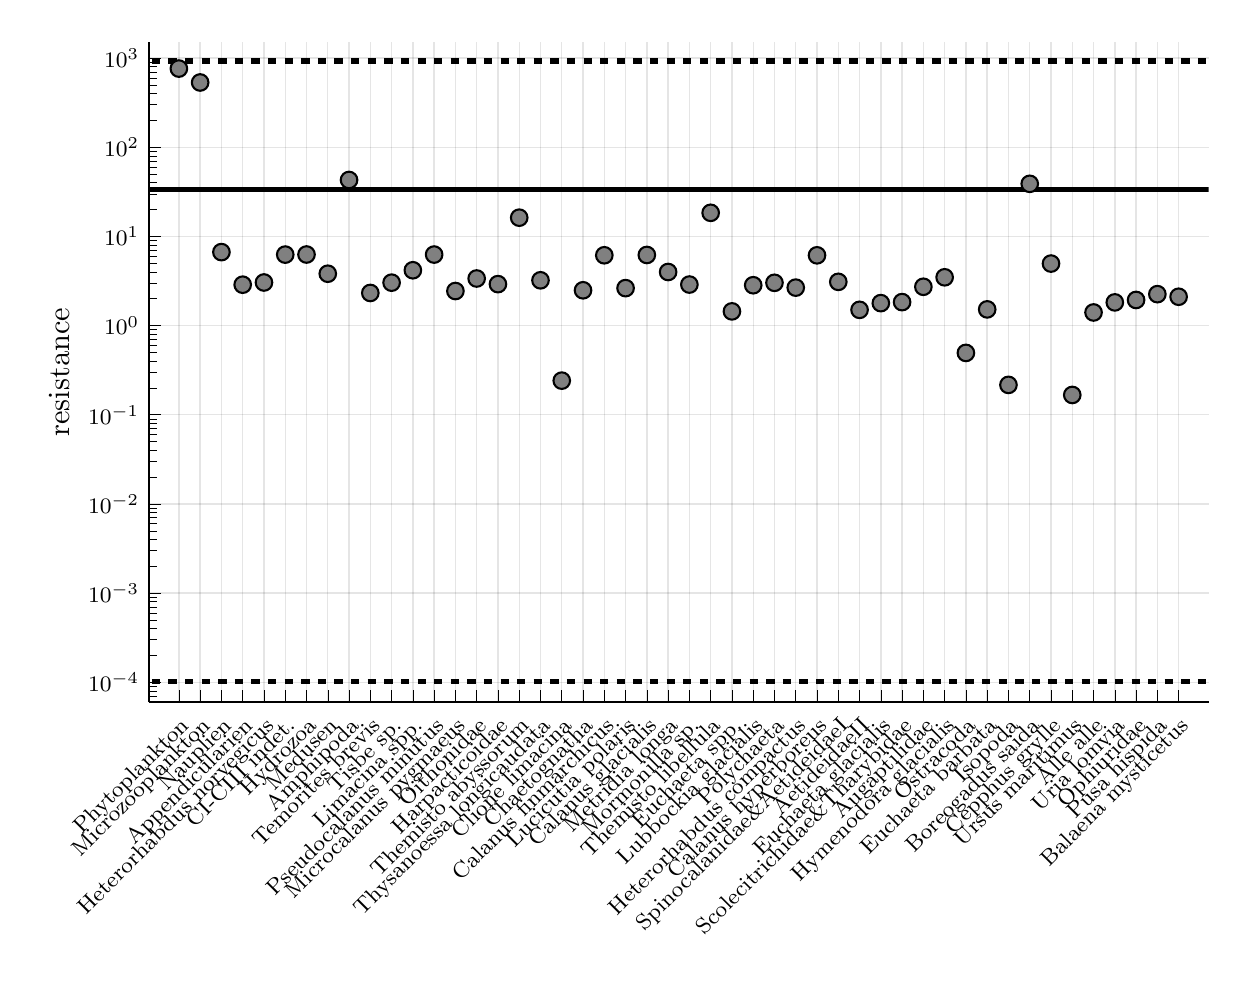
\begin{tikzpicture}[/tikz/background rectangle/.style={fill={rgb,1:red,1.0;green,1.0;blue,1.0}, fill opacity={1.0}, draw opacity={1.0}}, show background rectangle]
\begin{axis}[ymode = log, point meta max={nan}, point meta min={nan}, legend cell align={left}, legend columns={1}, title={}, title style={at={{(0.5,1)}}, anchor={south}, font={{\fontsize{14 pt}{18.2 pt}\selectfont}}, color={rgb,1:red,0.0;green,0.0;blue,0.0}, draw opacity={1.0}, rotate={0.0}, align={center}}, legend style={color={rgb,1:red,0.0;green,0.0;blue,0.0}, draw opacity={1.0}, line width={1}, solid, fill={rgb,1:red,1.0;green,1.0;blue,1.0}, fill opacity={1.0}, text opacity={1.0}, font={{\fontsize{8 pt}{10.4 pt}\selectfont}}, text={rgb,1:red,0.0;green,0.0;blue,0.0}, cells={anchor={center}}, at={(1.02, 1)}, anchor={north west}}, axis background/.style={fill={rgb,1:red,1.0;green,1.0;blue,1.0}, opacity={1.0}}, anchor={north west}, xshift={1.0mm}, yshift={-1.0mm}, width={150.4mm}, height={99.6mm}, scaled x ticks={false}, xlabel={}, x tick style={color={rgb,1:red,0.0;green,0.0;blue,0.0}, opacity={1.0}}, x tick label style={color={rgb,1:red,0.0;green,0.0;blue,0.0}, opacity={1.0}, rotate={45}}, xlabel style={at={(ticklabel cs:0.5)}, anchor=near ticklabel, at={{(ticklabel cs:0.5)}}, anchor={near ticklabel}, font={{\fontsize{11 pt}{14.3 pt}\selectfont}}, color={rgb,1:red,0.0;green,0.0;blue,0.0}, draw opacity={1.0}, rotate={0.0}}, xmajorgrids={true}, xmin={-0.41000000000000014}, xmax={49.41}, xticklabels={{Phytoplankton,Microzooplankton ,Nauplien ,Appendicularien,Heterorhabdus norvegicus,CI-CIII indet.,Hydrozoa,Medusen,Amphipoda,Temorites brevis,Tisbe sp.,Limacina spp. ,Pseudocalanus minutus,Microcalanus pygmaeus,Oithonidae,Harpacticoidae,Themisto abyssorum,Thysanoessa longicaudata,Clione limacina,Chaetognatha,Calanus finmarchicus,Lucicutia polaris,Calanus glacialis,Metridia longa,Mormonilla sp.,Themisto libellula,Euchaeta spp.,Lubbockia glacialis,Polychaeta,Heterorhabdus compactus,Calanus hyperboreus,Spinocalanidae\&AetideidaeI,AetideidaeII,Euchaeta glacialis ,Scolecitrichidae\&Tharybidae,Augaptilidae,Hymenodora glacialis,Ostracoda,Euchaeta barbata ,Isopoda,Boreogadus saida,Cepphus grylle,Ursus maritimus,Alle alle,Uria lomvia,Ophiuridae,Pusa hispida,Balaena mysticetus}}, xtick={{1,2,3,4,5,6,7,8,9,10,11,12,13,14,15,16,17,18,19,20,21,22,23,24,25,26,27,28,29,30,31,32,33,34,35,36,37,38,39,40,41,42,43,44,45,46,47,48}}, xtick align={inside}, xticklabel style={font={{\fontsize{8 pt}{10.4 pt}\selectfont}}, color={rgb,1:red,0.0;green,0.0;blue,0.0}, draw opacity={1.0}, rotate={0.0}, anchor={north east}}, x grid style={color={rgb,1:red,0.0;green,0.0;blue,0.0}, draw opacity={0.1}, line width={0.5}, solid}, axis x line*={left}, x axis line style={color={rgb,1:red,0.0;green,0.0;blue,0.0}, draw opacity={1.0}, line width={1}, solid}, scaled y ticks={false}, ylabel={resistance}, y tick style={color={rgb,1:red,0.0;green,0.0;blue,0.0}, opacity={1.0}}, y tick label style={color={rgb,1:red,0.0;green,0.0;blue,0.0}, opacity={1.0}, rotate={0}}, ylabel style={at={(ticklabel cs:0.5)}, anchor=near ticklabel, at={{(ticklabel cs:0.5)}}, anchor={near ticklabel}, font={{\fontsize{11 pt}{14.3 pt}\selectfont}}, color={rgb,1:red,0.0;green,0.0;blue,0.0}, draw opacity={1.0}, rotate={0.0}}, ymajorgrids={true}, ymin={0.00006}, ymax={1500},
%	 yticklabels={{0.0,min,expected,200.0,400.0,600.0,800.0,max}}, ytick={{0.0,0.0001023952561400688,33.431364950240926,200.0,400.0,600.0,800.0,924.7584151981167}}, 
	 ytick align={inside}, yticklabel style={font={{\fontsize{8 pt}{10.4 pt}\selectfont}}, color={rgb,1:red,0.0;green,0.0;blue,0.0}, draw opacity={1.0}, rotate={0.0}}, y grid style={color={rgb,1:red,0.0;green,0.0;blue,0.0}, draw opacity={0.1}, line width={0.5}, solid}, axis y line*={left}, y axis line style={color={rgb,1:red,0.0;green,0.0;blue,0.0}, draw opacity={1.0}, line width={1}, solid}, colorbar={false}]
    \addplot[color={rgb,1:red,0.502;green,0.502;blue,0.502}, name path={1}, only marks, draw opacity={1.0}, line width={0}, solid, mark={*}, mark size={3.0 pt}, mark repeat={1}, mark options={color={rgb,1:red,0.0;green,0.0;blue,0.0}, draw opacity={1.0}, fill={rgb,1:red,0.502;green,0.502;blue,0.502}, fill opacity={1.0}, line width={0.75}, rotate={0}, solid}]
        table[row sep={\\}]
        {
            \\
            1.0  762.48879994873  \\
            2.0  532.4626930418343  \\
            3.0  6.667397612605446  \\
            4.0  2.875957163064506  \\
            5.0  3.0435617452612154  \\
            6.0  6.254543217678066  \\
            7.0  6.269136720821746  \\
            8.0  3.817324175695607  \\
            9.0  42.92662660050886  \\
            10.0  2.322572281103009  \\
            11.0  3.0302234231222194  \\
            12.0  4.173548486528599  \\
            13.0  6.259626177035249  \\
            14.0  2.4416419396670976  \\
            15.0  3.3742564492316696  \\
            16.0  2.9173016929396525  \\
            17.0  16.22770109181183  \\
            18.0  3.2206148573690037  \\
            19.0  0.24142346980579063  \\
            20.0  2.4886796462485448  \\
            21.0  6.147012902415771  \\
            22.0  2.6313832047191816  \\
            23.0  6.195961845436984  \\
            24.0  3.991446055798839  \\
            25.0  2.886446536251632  \\
            26.0  18.394355144478453  \\
            27.0  1.4436235542973792  \\
            28.0  2.8356458959936037  \\
            29.0  3.018693803997041  \\
            30.0  2.665757871124397  \\
            31.0  6.138228386523896  \\
            32.0  3.09445076060905  \\
            33.0  1.5022692891987965  \\
            34.0  1.786129266772586  \\
            35.0  1.8337071687822226  \\
            36.0  2.7247122292842167  \\
            37.0  3.4804542320789524  \\
            38.0  0.4939363131527996  \\
            39.0  1.5196273520198806  \\
            40.0  0.21631433972923142  \\
            41.0  38.89468471576695  \\
            42.0  4.962086466462506  \\
            43.0  0.16682675673281291  \\
            44.0  1.4040792210172102  \\
            45.0  1.8204480230171907  \\
            46.0  1.9385336062417013  \\
            47.0  2.2517236774829437  \\
            48.0  2.1063997897111078  \\
        }
        ;
    \addplot[color={rgb,1:red,0.0;green,0.0;blue,0.0}, name path={2}, draw opacity={1.0}, line width={2}, dashed]
        table[row sep={\\}]
        {
            \\
            -50.22999999999999  0.0001023952561400688  \\
            99.22999999999999  0.0001023952561400688  \\
        }
        ;
    \addplot[color={rgb,1:red,0.0;green,0.0;blue,0.0}, name path={3}, draw opacity={1.0}, line width={2}, solid]
        table[row sep={\\}]
        {
            \\
            -50.22999999999999  33.431364950240926  \\
            99.22999999999999  33.431364950240926  \\
        }
        ;
    \addplot[color={rgb,1:red,0.0;green,0.0;blue,0.0}, name path={4}, draw opacity={1.0}, line width={2}, dashed]
        table[row sep={\\}]
        {
            \\
            -50.22999999999999  924.7584151981167  \\
            99.22999999999999  924.7584151981167  \\
        }
        ;
\end{axis}
\end{tikzpicture}

	}
	\caption{
		Minimal (dashed line bottom), maximal (dashed line top) end expected (solid line) value of resistance measure.
		Dots describe how resistant single species are within this range.
	}
\end{figure}
\begin{figure}
	\resizebox{\textwidth}{!}{
		% Recommended preamble:
% \usetikzlibrary{arrows.meta}
% \usetikzlibrary{backgrounds}
% \usepgfplotslibrary{patchplots}
% \usepgfplotslibrary{fillbetween}
% \pgfplotsset{%
%     layers/standard/.define layer set={%
%         background,axis background,axis grid,axis ticks,axis lines,axis tick labels,pre main,main,axis descriptions,axis foreground%
%     }{
%         grid style={/pgfplots/on layer=axis grid},%
%         tick style={/pgfplots/on layer=axis ticks},%
%         axis line style={/pgfplots/on layer=axis lines},%
%         label style={/pgfplots/on layer=axis descriptions},%
%         legend style={/pgfplots/on layer=axis descriptions},%
%         title style={/pgfplots/on layer=axis descriptions},%
%         colorbar style={/pgfplots/on layer=axis descriptions},%
%         ticklabel style={/pgfplots/on layer=axis tick labels},%
%         axis background@ style={/pgfplots/on layer=axis background},%
%         3d box foreground style={/pgfplots/on layer=axis foreground},%
%     },
% }

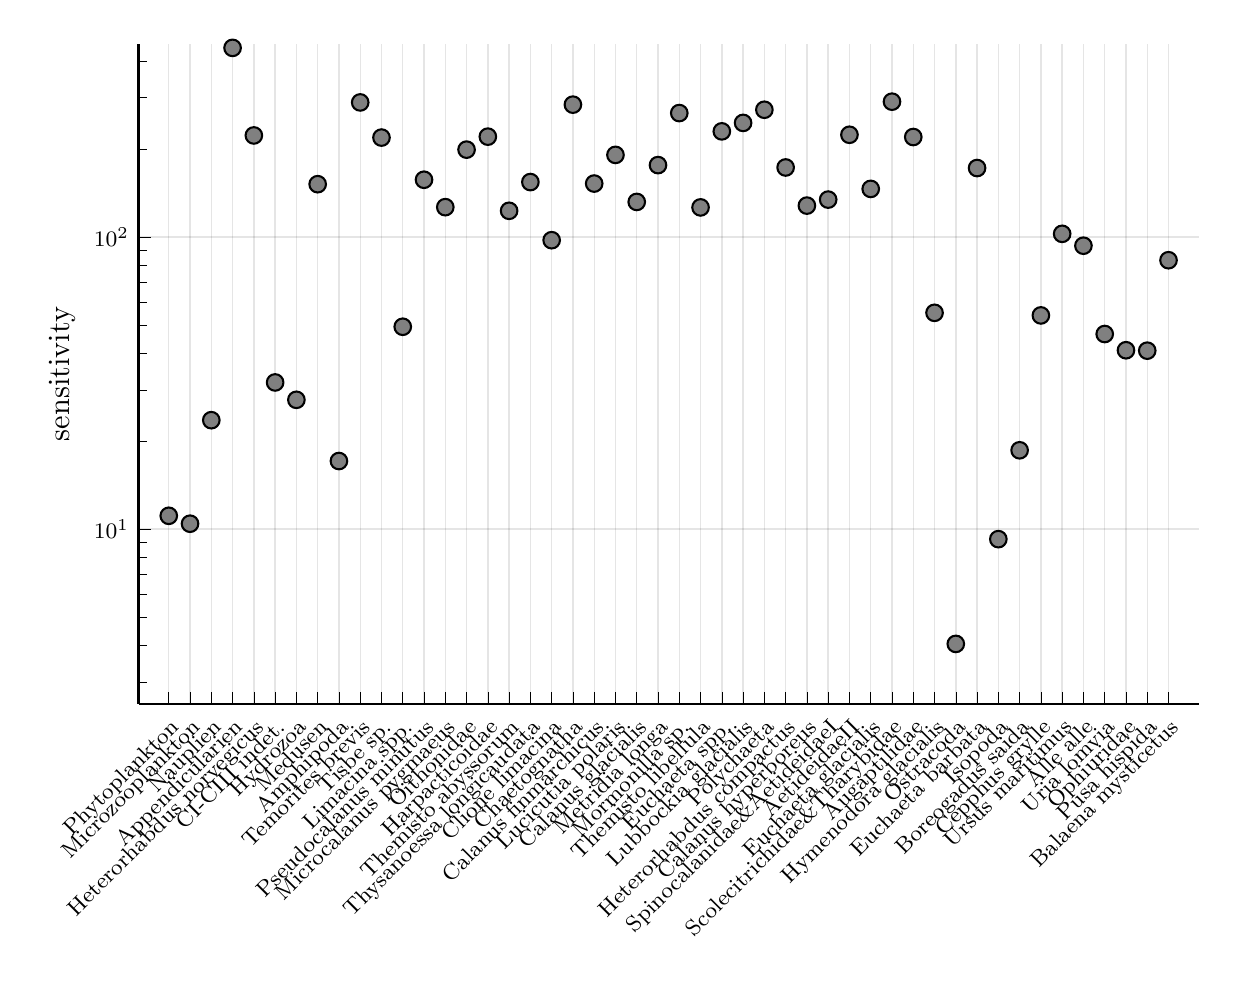
\begin{tikzpicture}[/tikz/background rectangle/.style={fill={rgb,1:red,1.0;green,1.0;blue,1.0}, fill opacity={1.0}, draw opacity={1.0}}, show background rectangle]
\begin{axis}[ymode = log, point meta max={nan}, point meta min={nan}, legend cell align={left}, legend columns={1}, title={}, title style={at={{(0.5,1)}}, anchor={south}, font={{\fontsize{14 pt}{18.2 pt}\selectfont}}, color={rgb,1:red,0.0;green,0.0;blue,0.0}, draw opacity={1.0}, rotate={0.0}, align={center}}, legend style={color={rgb,1:red,0.0;green,0.0;blue,0.0}, draw opacity={1.0}, line width={1}, solid, fill={rgb,1:red,1.0;green,1.0;blue,1.0}, fill opacity={1.0}, text opacity={1.0}, font={{\fontsize{8 pt}{10.4 pt}\selectfont}}, text={rgb,1:red,0.0;green,0.0;blue,0.0}, cells={anchor={center}}, at={(1.02, 1)}, anchor={north west}}, axis background/.style={fill={rgb,1:red,1.0;green,1.0;blue,1.0}, opacity={1.0}}, anchor={north west}, xshift={1.0mm}, yshift={-1.0mm}, width={150.4mm}, height={99.6mm}, scaled x ticks={false}, xlabel={}, x tick style={color={rgb,1:red,0.0;green,0.0;blue,0.0}, opacity={1.0}}, x tick label style={color={rgb,1:red,0.0;green,0.0;blue,0.0}, opacity={1.0}, rotate={45}}, xlabel style={at={(ticklabel cs:0.5)}, anchor=near ticklabel, at={{(ticklabel cs:0.5)}}, anchor={near ticklabel}, font={{\fontsize{11 pt}{14.3 pt}\selectfont}}, color={rgb,1:red,0.0;green,0.0;blue,0.0}, draw opacity={1.0}, rotate={0.0}}, xmajorgrids={true}, xmin={-0.41000000000000014}, xmax={49.41}, xticklabels={{Phytoplankton,Microzooplankton,Nauplien ,Appendicularien,Heterorhabdus norvegicus,CI-CIII indet. ,Hydrozoa,Medusen,Amphipoda,Temorites brevis,Tisbe sp.,Limacina spp. ,Pseudocalanus minutus,Microcalanus pygmaeus,Oithonidae,Harpacticoidae ,Themisto abyssorum,Thysanoessa longicaudata,Clione limacina,Chaetognatha,Calanus finmarchicus,Lucicutia polaris,Calanus glacialis,Metridia longa,Mormonilla sp.,Themisto libellula,Euchaeta spp.,Lubbockia glacialis,Polychaeta,Heterorhabdus compactus ,Calanus hyperboreus,Spinocalanidae\&AetideidaeI,AetideidaeII,Euchaeta glacialis,Scolecitrichidae\&Tharybidae,Augaptilidae,Hymenodora glacialis,Ostracoda,Euchaeta barbata ,Isopoda,Boreogadus saida,Cepphus grylle,Ursus maritimus,Alle alle,Uria lomvia,Ophiuridae,Pusa hispida,Balaena mysticetus}}, xtick={{1,2,3,4,5,6,7,8,9,10,11,12,13,14,15,16,17,18,19,20,21,22,23,24,25,26,27,28,29,30,31,32,33,34,35,36,37,38,39,40,41,42,43,44,45,46,47,48}}, xtick align={inside}, xticklabel style={font={{\fontsize{8 pt}{10.4 pt}\selectfont}}, color={rgb,1:red,0.0;green,0.0;blue,0.0}, draw opacity={1.0}, rotate={0.0}, anchor={north east}}, x grid style={color={rgb,1:red,0.0;green,0.0;blue,0.0}, draw opacity={0.1}, line width={0.5}, solid}, axis x line*={left}, x axis line style={color={rgb,1:red,0.0;green,0.0;blue,0.0}, draw opacity={1.0}, line width={1}, solid}, scaled y ticks={false}, ylabel={sensitivity}, y tick style={color={rgb,1:red,0.0;green,0.0;blue,0.0}, opacity={1.0}}, y tick label style={color={rgb,1:red,0.0;green,0.0;blue,0.0}, opacity={1.0}, rotate={0}}, ylabel style={at={(ticklabel cs:0.5)}, anchor=near ticklabel, at={{(ticklabel cs:0.5)}}, anchor={near ticklabel}, font={{\fontsize{11 pt}{14.3 pt}\selectfont}}, color={rgb,1:red,0.0;green,0.0;blue,0.0}, draw opacity={1.0}, rotate={0.0}}, ymajorgrids={true},
	 ymin={-9.148091363449623}, ymax={457.15284715022904},
%	  yticklabels={{$0$,$100$,$200$,$300$,$400$}}, ytick={{0.0,100.0,200.0,300.0,400.0}},
	   ytick align={inside}, yticklabel style={font={{\fontsize{8 pt}{10.4 pt}\selectfont}}, color={rgb,1:red,0.0;green,0.0;blue,0.0}, draw opacity={1.0}, rotate={0.0}}, y grid style={color={rgb,1:red,0.0;green,0.0;blue,0.0}, draw opacity={0.1}, line width={0.5}, solid}, axis y line*={left}, y axis line style={color={rgb,1:red,0.0;green,0.0;blue,0.0}, draw opacity={1.0}, line width={1}, solid}, colorbar={false}]
    \addplot[color={rgb,1:red,0.502;green,0.502;blue,0.502}, name path={17}, only marks, draw opacity={1.0}, line width={0}, solid, mark={*}, mark size={3.0 pt}, mark repeat={1}, mark options={color={rgb,1:red,0.0;green,0.0;blue,0.0}, draw opacity={1.0}, fill={rgb,1:red,0.502;green,0.502;blue,0.502}, fill opacity={1.0}, line width={0.75}, rotate={0}, solid}]
        table[row sep={\\}]
        {
            \\
            1.0  11.112879880099964  \\
            2.0  10.441644143989047  \\
            3.0  23.607403794106823  \\
            4.0  443.9556507772004  \\
            5.0  222.65298233223945  \\
            6.0  31.78568553806307  \\
            7.0  27.721493961155684  \\
            8.0  151.63942936380008  \\
            9.0  17.112542927186915  \\
            10.0  288.8382621767416  \\
            11.0  218.93077878019673  \\
            12.0  49.29920998515056  \\
            13.0  157.0399100326077  \\
            14.0  126.52983525422151  \\
            15.0  199.12530195747559  \\
            16.0  220.56190619769905  \\
            17.0  122.9488604781985  \\
            18.0  154.1887761552247  \\
            19.0  97.52097726517584  \\
            20.0  283.82186595045874  \\
            21.0  152.40304623679248  \\
            22.0  191.02255900511418  \\
            23.0  131.84547557771316  \\
            24.0  176.25758990280508  \\
            25.0  265.60107793473856  \\
            26.0  126.2840543683594  \\
            27.0  229.93211713375226  \\
            28.0  245.78552213968263  \\
            29.0  272.6099160507052  \\
            30.0  172.99741867850562  \\
            31.0  128.08723904728305  \\
            32.0  134.30527109222996  \\
            33.0  223.86693174778813  \\
            34.0  146.1094402294383  \\
            35.0  290.5439099342536  \\
            36.0  219.93305282405854  \\
            37.0  55.02148867965704  \\
            38.0  4.049105009579034  \\
            39.0  172.21823483607542  \\
            40.0  9.245804057666605  \\
            41.0  18.624782488397475  \\
            42.0  53.91023187928788  \\
            43.0  102.53772168471687  \\
            44.0  93.37321359783543  \\
            45.0  46.558190228183406  \\
            46.0  40.96828995877132  \\
            47.0  40.834886852145694  \\
            48.0  83.28509093658657  \\
        }
        ;
\end{axis}
\end{tikzpicture}

	}
	\caption{
		Sensitivity of each species.
	}
\end{figure}

Interpretation: The abundance of most species is more easily manipulated than a random combination. This measure is based on the controllability Gramian.\pagebreak


\begin{figure}
	\resizebox{\textwidth}{!}{
		% Recommended preamble:
% \usetikzlibrary{arrows.meta}
% \usetikzlibrary{backgrounds}
% \usepgfplotslibrary{patchplots}
% \usepgfplotslibrary{fillbetween}
% \pgfplotsset{%
%     layers/standard/.define layer set={%
%         background,axis background,axis grid,axis ticks,axis lines,axis tick labels,pre main,main,axis descriptions,axis foreground%
%     }{
%         grid style={/pgfplots/on layer=axis grid},%
%         tick style={/pgfplots/on layer=axis ticks},%
%         axis line style={/pgfplots/on layer=axis lines},%
%         label style={/pgfplots/on layer=axis descriptions},%
%         legend style={/pgfplots/on layer=axis descriptions},%
%         title style={/pgfplots/on layer=axis descriptions},%
%         colorbar style={/pgfplots/on layer=axis descriptions},%
%         ticklabel style={/pgfplots/on layer=axis tick labels},%
%         axis background@ style={/pgfplots/on layer=axis background},%
%         3d box foreground style={/pgfplots/on layer=axis foreground},%
%     },
% }

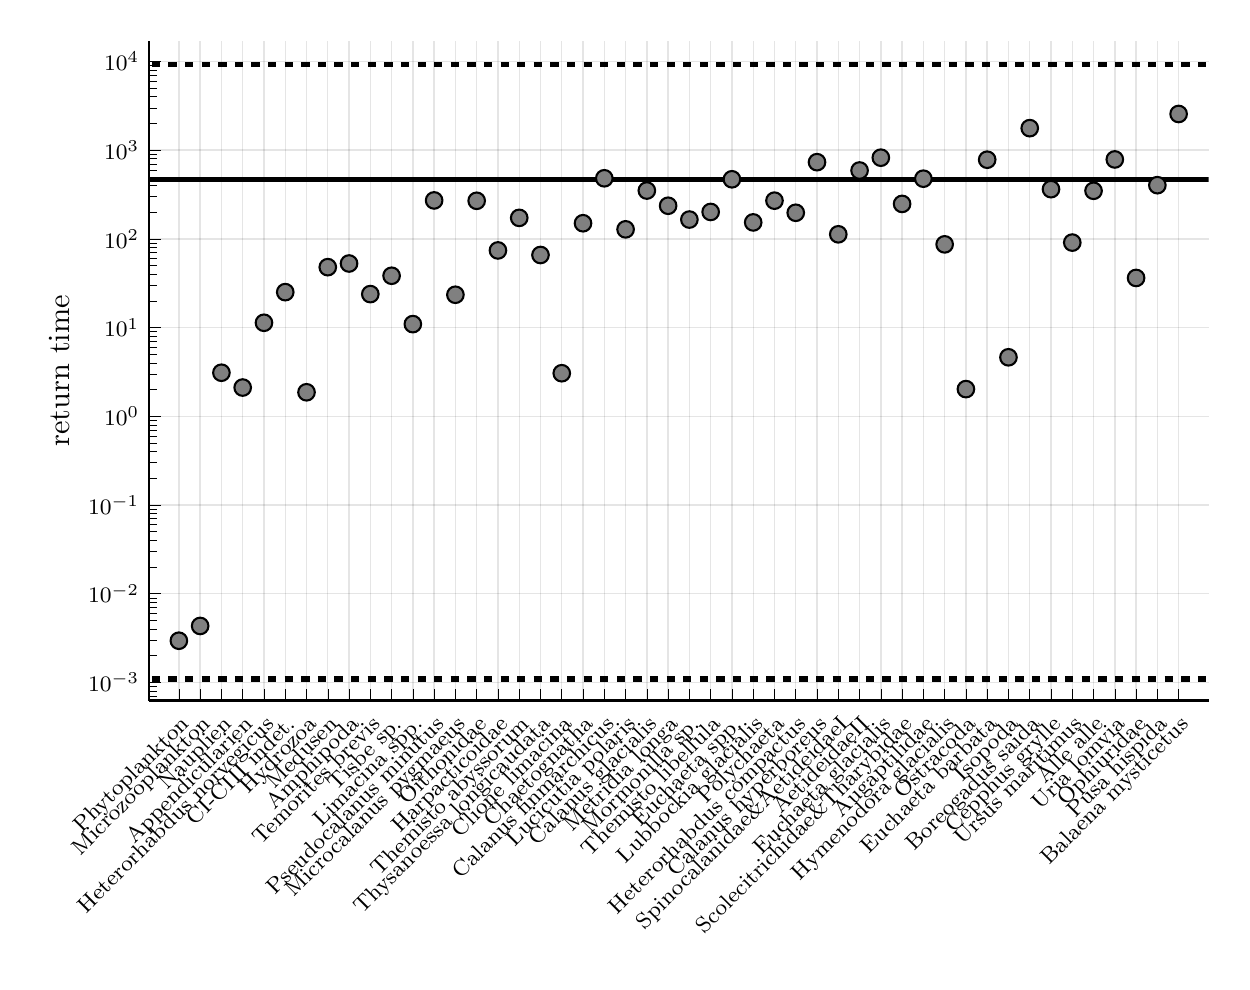
\begin{tikzpicture}[/tikz/background rectangle/.style={fill={rgb,1:red,1.0;green,1.0;blue,1.0}, fill opacity={1.0}, draw opacity={1.0}}, show background rectangle]
\begin{axis}[ymode = log, point meta max={nan}, point meta min={nan}, legend cell align={left}, legend columns={1}, title={}, title style={at={{(0.5,1)}}, anchor={south}, font={{\fontsize{14 pt}{18.2 pt}\selectfont}}, color={rgb,1:red,0.0;green,0.0;blue,0.0}, draw opacity={1.0}, rotate={0.0}, align={center}}, legend style={color={rgb,1:red,0.0;green,0.0;blue,0.0}, draw opacity={1.0}, line width={1}, solid, fill={rgb,1:red,1.0;green,1.0;blue,1.0}, fill opacity={1.0}, text opacity={1.0}, font={{\fontsize{8 pt}{10.4 pt}\selectfont}}, text={rgb,1:red,0.0;green,0.0;blue,0.0}, cells={anchor={center}}, at={(1.02, 1)}, anchor={north west}}, axis background/.style={fill={rgb,1:red,1.0;green,1.0;blue,1.0}, opacity={1.0}}, anchor={north west}, xshift={1.0mm}, yshift={-1.0mm}, width={150.4mm}, height={99.6mm}, scaled x ticks={false}, xlabel={}, x tick style={color={rgb,1:red,0.0;green,0.0;blue,0.0}, opacity={1.0}}, x tick label style={color={rgb,1:red,0.0;green,0.0;blue,0.0}, opacity={1.0}, rotate={45}}, xlabel style={at={(ticklabel cs:0.5)}, anchor=near ticklabel, at={{(ticklabel cs:0.5)}}, anchor={near ticklabel}, font={{\fontsize{11 pt}{14.3 pt}\selectfont}}, color={rgb,1:red,0.0;green,0.0;blue,0.0}, draw opacity={1.0}, rotate={0.0}}, xmajorgrids={true}, xmin={-0.41000000000000014}, xmax={49.41}, xticklabels={{Phytoplankton,Microzooplankton  ,Nauplien ,Appendicularien,Heterorhabdus norvegicus,CI-CIII indet.,Hydrozoa, Medusen,Amphipoda,Temorites brevis,Tisbe sp.,Limacina spp. ,Pseudocalanus minutus,Microcalanus pygmaeus,Oithonidae,Harpacticoidae ,Themisto abyssorum,Thysanoessa longicaudata,Clione limacina,Chaetognatha,Calanus finmarchicus,Lucicutia polaris,Calanus glacialis,Metridia longa,Mormonilla sp.,Themisto libellula,Euchaeta spp.,Lubbockia glacialis,Polychaeta,Heterorhabdus compactus,Calanus hyperboreus,Spinocalanidae\&AetideidaeI,AetideidaeII,Euchaeta glacialis,Scolecitrichidae\&Tharybidae,Augaptilidae,Hymenodora glacialis,Ostracoda,Euchaeta barbata ,Isopoda,Boreogadus saida,Cepphus grylle,Ursus maritimus,Alle alle,Uria lomvia,Ophiuridae,Pusa hispida,Balaena mysticetus}}, xtick={{1,2,3,4,5,6,7,8,9,10,11,12,13,14,15,16,17,18,19,20,21,22,23,24,25,26,27,28,29,30,31,32,33,34,35,36,37,38,39,40,41,42,43,44,45,46,47,48}}, xtick align={inside}, xticklabel style={font={{\fontsize{8 pt}{10.4 pt}\selectfont}}, color={rgb,1:red,0.0;green,0.0;blue,0.0}, draw opacity={1.0}, rotate={0.0}, anchor={north east}}, x grid style={color={rgb,1:red,0.0;green,0.0;blue,0.0}, draw opacity={0.1}, line width={0.5}, solid}, axis x line*={left}, x axis line style={color={rgb,1:red,0.0;green,0.0;blue,0.0}, draw opacity={1.0}, line width={1}, solid}, scaled y ticks={false}, ylabel={return time}, y tick style={color={rgb,1:red,0.0;green,0.0;blue,0.0}, opacity={1.0}}, y tick label style={color={rgb,1:red,0.0;green,0.0;blue,0.0}, opacity={1.0}, rotate={0}}, ylabel style={at={(ticklabel cs:0.5)}, anchor=near ticklabel, at={{(ticklabel cs:0.5)}}, anchor={near ticklabel}, font={{\fontsize{11 pt}{14.3 pt}\selectfont}}, color={rgb,1:red,0.0;green,0.0;blue,0.0}, draw opacity={1.0}, rotate={0.0}}, ymajorgrids={true}, ymin={-277.2652583659601}, ymax={17000}, 
%	yticklabels={{0.0,min,expected,2000.0,4000.0,6000.0,8000.0,max}}, ytick={{0.0,0.0010930925902669444,464.86495605342304,2000.0,4000.0,6000.0,8000.0,9242.212808377613}},
	 ytick align={inside}, yticklabel style={font={{\fontsize{8 pt}{10.4 pt}\selectfont}}, color={rgb,1:red,0.0;green,0.0;blue,0.0}, draw opacity={1.0}, rotate={0.0}}, y grid style={color={rgb,1:red,0.0;green,0.0;blue,0.0}, draw opacity={0.1}, line width={0.5}, solid}, axis y line*={left}, y axis line style={color={rgb,1:red,0.0;green,0.0;blue,0.0}, draw opacity={1.0}, line width={1}, solid}, colorbar={false}]
    \addplot[color={rgb,1:red,0.502;green,0.502;blue,0.502}, name path={5}, only marks, draw opacity={1.0}, line width={0}, solid, mark={*}, mark size={3.0 pt}, mark repeat={1}, mark options={color={rgb,1:red,0.0;green,0.0;blue,0.0}, draw opacity={1.0}, fill={rgb,1:red,0.502;green,0.502;blue,0.502}, fill opacity={1.0}, line width={0.75}, rotate={0}, solid}]
        table[row sep={\\}]
        {
            \\
            1.0  0.002953093882987956  \\
            2.0  0.004331298593078437  \\
            3.0  3.0968951656358548  \\
            4.0  2.1081709339022296  \\
            5.0  11.325725233417884  \\
            6.0  25.076273782963398  \\
            7.0  1.8642198498331521  \\
            8.0  47.969090258354036  \\
            9.0  52.73928680252467  \\
            10.0  23.83495955491073  \\
            11.0  38.37204425933356  \\
            12.0  10.935377670493038  \\
            13.0  271.1059714695633  \\
            14.0  23.43141576313335  \\
            15.0  268.57288156661065  \\
            16.0  74.03933261018993  \\
            17.0  172.33450931692045  \\
            18.0  65.76605009871142  \\
            19.0  3.057287178285813  \\
            20.0  149.95324362947937  \\
            21.0  481.4704711109947  \\
            22.0  127.98200931728263  \\
            23.0  350.3572308390785  \\
            24.0  236.13292417823715  \\
            25.0  165.03398892985894  \\
            26.0  201.01188562732634  \\
            27.0  469.11488969566796  \\
            28.0  153.24117633854695  \\
            29.0  269.4523293360272  \\
            30.0  196.84006156520732  \\
            31.0  731.547642111958  \\
            32.0  112.4969716275462  \\
            33.0  589.475266981318  \\
            34.0  821.9411905994622  \\
            35.0  247.59453280647543  \\
            36.0  476.5724430105207  \\
            37.0  86.65560807021856  \\
            38.0  2.0245525047895176  \\
            39.0  779.88112619546  \\
            40.0  4.622902028833302  \\
            41.0  1769.2309287247972  \\
            42.0  362.97279483297666  \\
            43.0  90.74001827415395  \\
            44.0  348.14369071558775  \\
            45.0  785.5030792444962  \\
            46.0  36.25293981131779  \\
            47.0  402.64024372971716  \\
            48.0  2555.5103946032827  \\
        }
        ;
    \addplot[color={rgb,1:red,0.0;green,0.0;blue,0.0}, name path={6}, draw opacity={1.0}, line width={2}, dashed]
        table[row sep={\\}]
        {
            \\
            -50.22999999999999  0.0010930925902669444  \\
            99.22999999999999  0.0010930925902669444  \\
        }
        ;
    \addplot[color={rgb,1:red,0.0;green,0.0;blue,0.0}, name path={7}, draw opacity={1.0}, line width={2}, solid]
        table[row sep={\\}]
        {
            \\
            -50.22999999999999  464.86495605342304  \\
            99.22999999999999  464.86495605342304  \\
        }
        ;
    \addplot[color={rgb,1:red,0.0;green,0.0;blue,0.0}, name path={8}, draw opacity={1.0}, line width={2}, dashed]
        table[row sep={\\}]
        {
            \\
            -50.22999999999999  9242.212808377613  \\
            99.22999999999999  9242.212808377613  \\
        }
        ;
\end{axis}
\end{tikzpicture}

	}
	\caption{
		Minimal (dashed line bottom), maximal (dashed line top) end expected (solid line) value of return time measure.
		Dots describe the return time of the system within this range if only a single species is perturbed. 
	}
\end{figure}

Interpretation: Measure is based on the observability Gramian. It seems like the return time scales with turnover rate. When Phyto- or Mezoplankton is perturbed, the system returns fastest to the equilibrium. A pulse perturbation of Baleana mysticetus (lives above 100 years) yields a long return time.

\begin{figure}
	\resizebox{\textwidth}{!}{
		% Recommended preamble:
% \usetikzlibrary{arrows.meta}
% \usetikzlibrary{backgrounds}
% \usepgfplotslibrary{patchplots}
% \usepgfplotslibrary{fillbetween}
% \pgfplotsset{%
%     layers/standard/.define layer set={%
%         background,axis background,axis grid,axis ticks,axis lines,axis tick labels,pre main,main,axis descriptions,axis foreground%
%     }{
%         grid style={/pgfplots/on layer=axis grid},%
%         tick style={/pgfplots/on layer=axis ticks},%
%         axis line style={/pgfplots/on layer=axis lines},%
%         label style={/pgfplots/on layer=axis descriptions},%
%         legend style={/pgfplots/on layer=axis descriptions},%
%         title style={/pgfplots/on layer=axis descriptions},%
%         colorbar style={/pgfplots/on layer=axis descriptions},%
%         ticklabel style={/pgfplots/on layer=axis tick labels},%
%         axis background@ style={/pgfplots/on layer=axis background},%
%         3d box foreground style={/pgfplots/on layer=axis foreground},%
%     },
% }

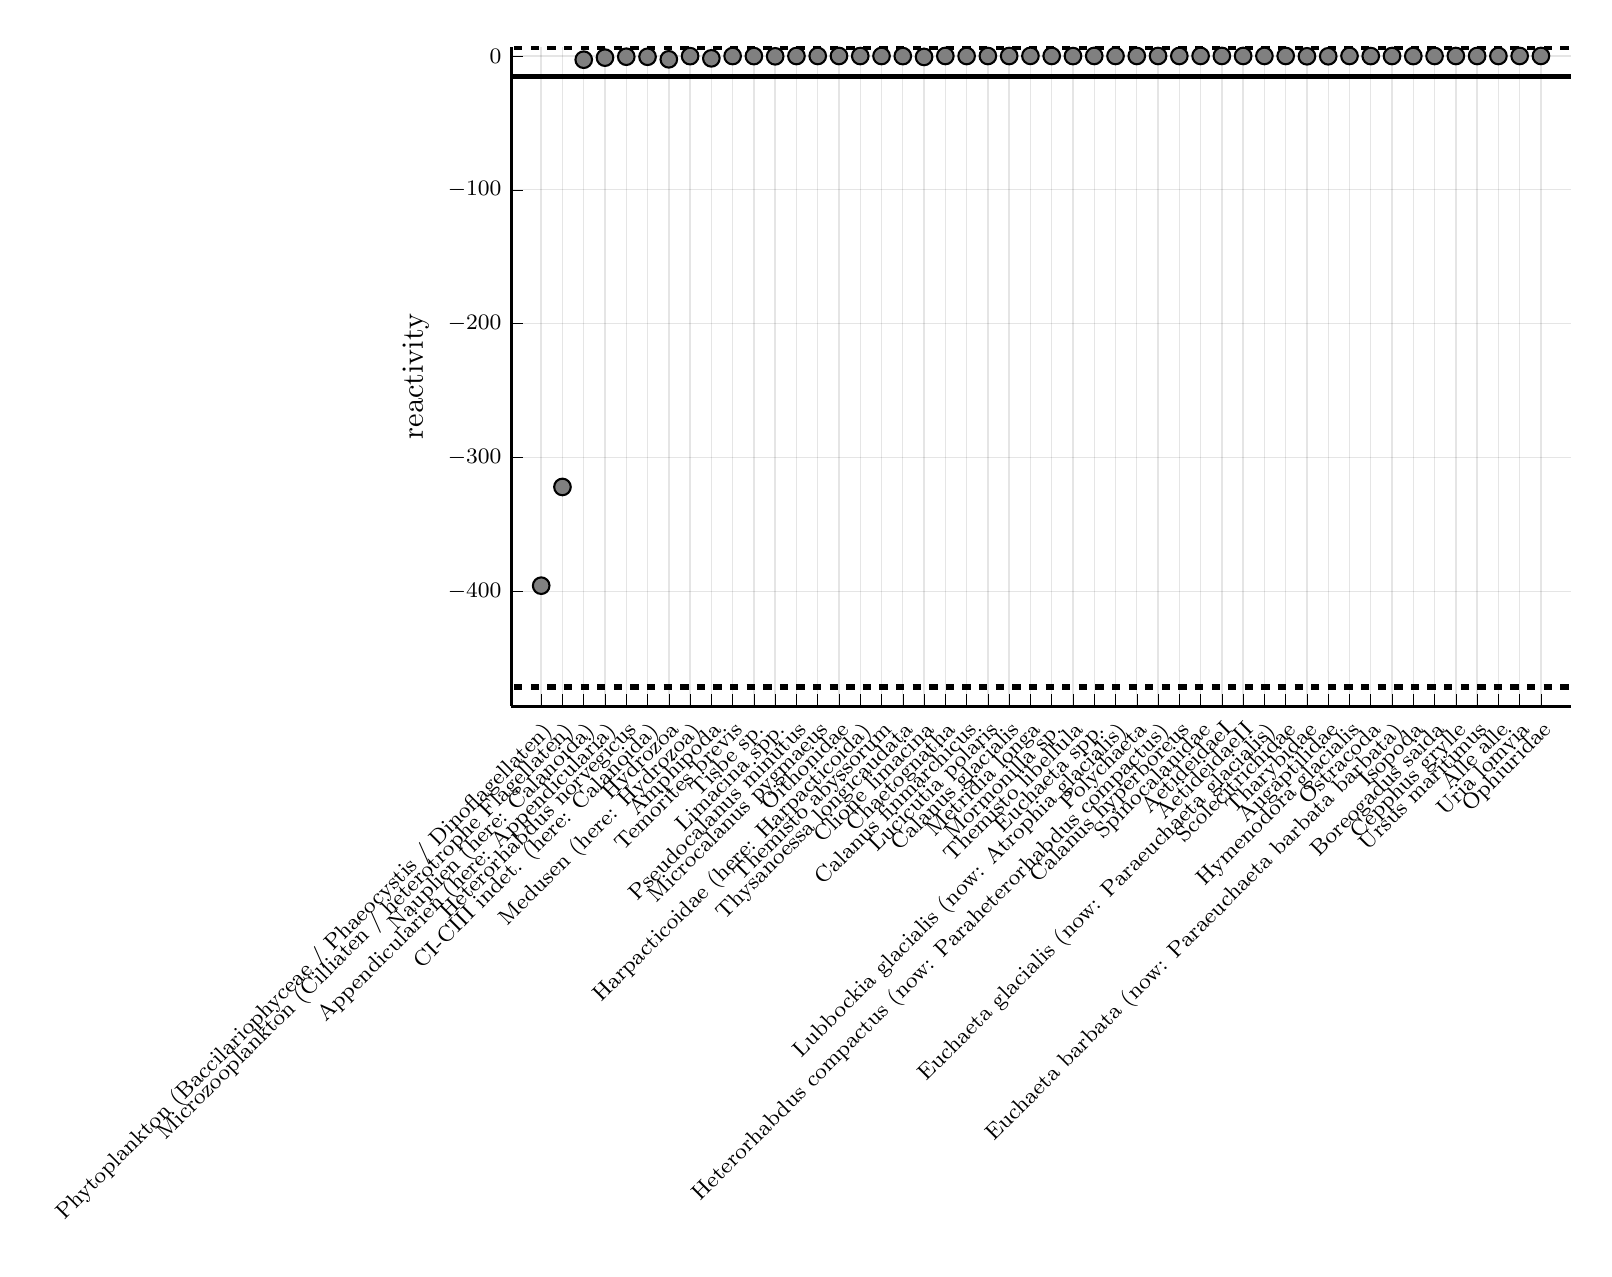
\begin{tikzpicture}[/tikz/background rectangle/.style={fill={rgb,1:red,1.0;green,1.0;blue,1.0}, fill opacity={1.0}, draw opacity={1.0}}, show background rectangle]
\begin{axis}[point meta max={nan}, point meta min={nan}, legend cell align={left}, legend columns={1}, title={}, title style={at={{(0.5,1)}}, anchor={south}, font={{\fontsize{14 pt}{18.2 pt}\selectfont}}, color={rgb,1:red,0.0;green,0.0;blue,0.0}, draw opacity={1.0}, rotate={0.0}, align={center}}, legend style={color={rgb,1:red,0.0;green,0.0;blue,0.0}, draw opacity={1.0}, line width={1}, solid, fill={rgb,1:red,1.0;green,1.0;blue,1.0}, fill opacity={1.0}, text opacity={1.0}, font={{\fontsize{8 pt}{10.4 pt}\selectfont}}, text={rgb,1:red,0.0;green,0.0;blue,0.0}, cells={anchor={center}}, at={(1.02, 1)}, anchor={north west}}, axis background/.style={fill={rgb,1:red,1.0;green,1.0;blue,1.0}, opacity={1.0}}, anchor={north west}, xshift={1.0mm}, yshift={-1.0mm}, width={150.4mm}, height={99.6mm}, scaled x ticks={false}, xlabel={}, x tick style={color={rgb,1:red,0.0;green,0.0;blue,0.0}, opacity={1.0}}, x tick label style={color={rgb,1:red,0.0;green,0.0;blue,0.0}, opacity={1.0}, rotate={45}}, xlabel style={at={(ticklabel cs:0.5)}, anchor=near ticklabel, at={{(ticklabel cs:0.5)}}, anchor={near ticklabel}, font={{\fontsize{11 pt}{14.3 pt}\selectfont}}, color={rgb,1:red,0.0;green,0.0;blue,0.0}, draw opacity={1.0}, rotate={0.0}}, xmajorgrids={true}, xmin={-0.41000000000000014}, xmax={49.41}, xticklabels={{Phytoplankton (Baccilariophyceae / Phaeocystis / Dinoflagellaten),Microzooplankton (Cilliaten / heterotrophe Flagellaten) ,Nauplien (here: Calanoida),Appendicularien (here: Appendicularia),Heterorhabdus norvegicus,CI-CIII indet. (here: Calanoida),Hydrozoa,Medusen (here: Hydrozoa),Amphipoda,Temorites brevis,Tisbe sp.,Limacina spp. ,Pseudocalanus minutus,Microcalanus pygmaeus,Oithonidae,Harpacticoidae (here: Harpacticoida),Themisto abyssorum,Thysanoessa longicaudata,Clione limacina,Chaetognatha,Calanus finmarchicus,Lucicutia polaris,Calanus glacialis,Metridia longa,Mormonilla sp.,Themisto libellula,Euchaeta spp.,Lubbockia glacialis (now: Atrophia glacialis),Polychaeta,Heterorhabdus compactus (now: Paraheterorhabdus compactus),Calanus hyperboreus,Spinocalanidae, AetideidaeI,AetideidaeII,Euchaeta glacialis (now: Paraeuchaeta glacialis),Scolecitrichidae, Tharybidae,Augaptilidae,Hymenodora glacialis,Ostracoda,Euchaeta barbata (now: Paraeuchaeta barbata barbata),Isopoda,Boreogadus saida,Cepphus grylle,Ursus maritimus,Alle alle,Uria lomvia,Ophiuridae,Pusa hispida,Balaena mysticetus}}, xtick={{1,2,3,4,5,6,7,8,9,10,11,12,13,14,15,16,17,18,19,20,21,22,23,24,25,26,27,28,29,30,31,32,33,34,35,36,37,38,39,40,41,42,43,44,45,46,47,48}}, xtick align={inside}, xticklabel style={font={{\fontsize{8 pt}{10.4 pt}\selectfont}}, color={rgb,1:red,0.0;green,0.0;blue,0.0}, draw opacity={1.0}, rotate={0.0}, anchor={north east}}, x grid style={color={rgb,1:red,0.0;green,0.0;blue,0.0}, draw opacity={0.1}, line width={0.5}, solid}, axis x line*={left}, x axis line style={color={rgb,1:red,0.0;green,0.0;blue,0.0}, draw opacity={1.0}, line width={1}, solid}, scaled y ticks={false}, ylabel={reactivity}, y tick style={color={rgb,1:red,0.0;green,0.0;blue,0.0}, opacity={1.0}}, y tick label style={color={rgb,1:red,0.0;green,0.0;blue,0.0}, opacity={1.0}, rotate={0}}, ylabel style={at={(ticklabel cs:0.5)}, anchor=near ticklabel, at={{(ticklabel cs:0.5)}}, anchor={near ticklabel}, font={{\fontsize{11 pt}{14.3 pt}\selectfont}}, color={rgb,1:red,0.0;green,0.0;blue,0.0}, draw opacity={1.0}, rotate={0.0}}, ymajorgrids={true}, 
	ymin={-485.8637401570752},
%	ymin={-16},
	ymax={7},
%	 ymax={20.958676863685554},
%	  yticklabels={{min,-400.0,-300.0,-200.0,-100.0,expected,0.0,max}},
%	   ytick={{-471.51970948667633,-400.0,-300.0,-200.0,-100.0,-15.288110869418341,0.0,6.6146461932866725}},
	    ytick align={inside}, yticklabel style={font={{\fontsize{8 pt}{10.4 pt}\selectfont}}, color={rgb,1:red,0.0;green,0.0;blue,0.0}, draw opacity={1.0}, rotate={0.0}}, y grid style={color={rgb,1:red,0.0;green,0.0;blue,0.0}, draw opacity={0.1}, line width={0.5}, solid}, axis y line*={left}, y axis line style={color={rgb,1:red,0.0;green,0.0;blue,0.0}, draw opacity={1.0}, line width={1}, solid}, colorbar={false}]
    \addplot[color={rgb,1:red,0.502;green,0.502;blue,0.502}, name path={1}, only marks, draw opacity={1.0}, line width={0}, solid, mark={*}, mark size={3.0 pt}, mark repeat={1}, mark options={color={rgb,1:red,0.0;green,0.0;blue,0.0}, draw opacity={1.0}, fill={rgb,1:red,0.502;green,0.502;blue,0.502}, fill opacity={1.0}, line width={0.75}, rotate={0}, solid}]
        table[row sep={\\}]
        {
            \\
            1.0  -395.74937866361637  \\
            2.0  -321.9944056184741  \\
            3.0  -2.8123725878574906  \\
            4.0  -1.2761971376119081  \\
            5.0  -0.5784943665843791  \\
            6.0  -0.6246526948262466  \\
            7.0  -2.5265665336125243  \\
            8.0  -0.16196679193338043  \\
            9.0  -1.7997435198577727  \\
            10.0  -0.084931556014448  \\
            11.0  -0.1167517681432196  \\
            12.0  -0.28463434052993136  \\
            13.0  -0.07036582484541183  \\
            14.0  -0.033770676489106755  \\
            15.0  -0.04032571875775379  \\
            16.0  -0.06438376674908655  \\
            17.0  -0.05784224300109236  \\
            18.0  -0.11972955928416514  \\
            19.0  -0.7400142505654593  \\
            20.0  -0.03451350084380774  \\
            21.0  -0.05952526273750033  \\
            22.0  -0.04451746873529337  \\
            23.0  -0.05458315095736466  \\
            24.0  0.02702738629563282  \\
            25.0  -0.03017955553317447  \\
            26.0  -0.10749827811722525  \\
            27.0  -0.010934801632810838  \\
            28.0  -0.027883436538519924  \\
            29.0  -0.023347767832630074  \\
            30.0  -0.026464544768720073  \\
            31.0  -0.028017324040878405  \\
            32.0  -0.0075973127640222345  \\
            33.0  -0.014709814481957045  \\
            34.0  -0.022678409779969613  \\
            35.0  -0.01488003280120044  \\
            36.0  -0.015383411715914546  \\
            37.0  -0.2546341913972188  \\
            38.0  -0.24351613625282104  \\
            39.0  -0.01581929289779308  \\
            40.0  -0.10753782591294407  \\
            41.0  -0.0539846403336853  \\
            42.0  -0.09615099442402737  \\
            43.0  -0.04788062466677963  \\
            44.0  -0.03575407287267078  \\
            45.0  -0.03631280705506143  \\
            46.0  -0.03359806484520137  \\
            47.0  -0.0184297035895433  \\
            48.0  -0.009664032999503528  \\
        }
        ;
    \addplot[color={rgb,1:red,0.0;green,0.0;blue,0.0}, name path={2}, draw opacity={1.0}, line width={2}, dashed]
        table[row sep={\\}]
        {
            \\
            -50.22999999999999  -471.51970948667633  \\
            99.22999999999999  -471.51970948667633  \\
        }
        ;
    \addplot[color={rgb,1:red,0.0;green,0.0;blue,0.0}, name path={3}, draw opacity={1.0}, line width={2}, solid]
        table[row sep={\\}]
        {
            \\
            -50.22999999999999  -15.288110869418341  \\
            99.22999999999999  -15.288110869418341  \\
        }
        ;
    \addplot[color={rgb,1:red,0.0;green,0.0;blue,0.0}, name path={4}, draw opacity={1.0}, line width={2}, dashed]
        table[row sep={\\}]
        {
            \\
            -50.22999999999999  6.6146461932866725  \\
            99.22999999999999  6.6146461932866725  \\
        }
        ;
\end{axis}
\end{tikzpicture}

	}
	\caption{
		Need to work on this. There is obviously a bug in the code, as the dots should not lie outside the dashed bounds.
	}
\end{figure}

\begin{figure}
	\resizebox{\textwidth}{!}{
		% Recommended preamble:
% \usetikzlibrary{arrows.meta}
% \usetikzlibrary{backgrounds}
% \usepgfplotslibrary{patchplots}
% \usepgfplotslibrary{fillbetween}
% \pgfplotsset{%
%     layers/standard/.define layer set={%
%         background,axis background,axis grid,axis ticks,axis lines,axis tick labels,pre main,main,axis descriptions,axis foreground%
%     }{
%         grid style={/pgfplots/on layer=axis grid},%
%         tick style={/pgfplots/on layer=axis ticks},%
%         axis line style={/pgfplots/on layer=axis lines},%
%         label style={/pgfplots/on layer=axis descriptions},%
%         legend style={/pgfplots/on layer=axis descriptions},%
%         title style={/pgfplots/on layer=axis descriptions},%
%         colorbar style={/pgfplots/on layer=axis descriptions},%
%         ticklabel style={/pgfplots/on layer=axis tick labels},%
%         axis background@ style={/pgfplots/on layer=axis background},%
%         3d box foreground style={/pgfplots/on layer=axis foreground},%
%     },
% }

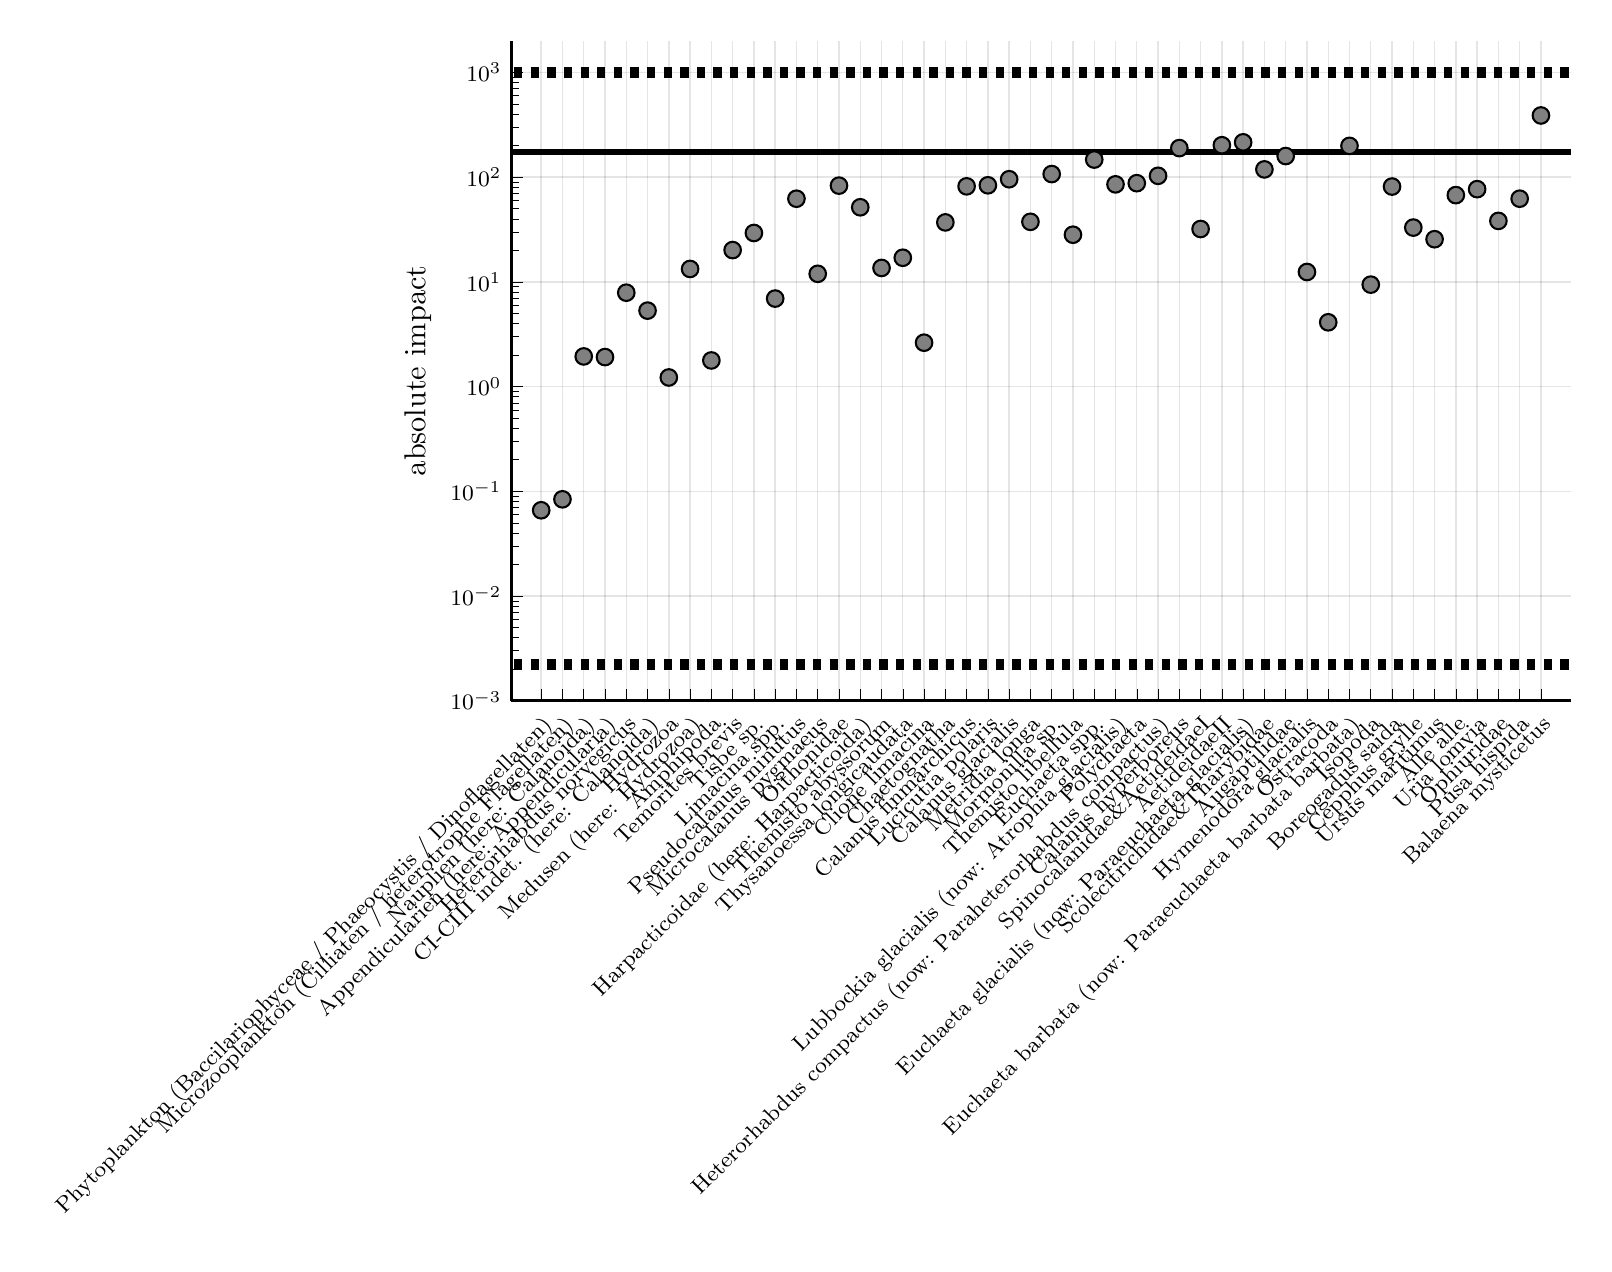
\begin{tikzpicture}[/tikz/background rectangle/.style={fill={rgb,1:red,1.0;green,1.0;blue,1.0}, fill opacity={1.0}, draw opacity={1.0}}, show background rectangle]
\begin{axis}[ymode =log, point meta max={nan}, point meta min={nan}, legend cell align={left}, legend columns={1}, title={}, title style={at={{(0.5,1)}}, anchor={south}, font={{\fontsize{14 pt}{18.2 pt}\selectfont}}, color={rgb,1:red,0.0;green,0.0;blue,0.0}, draw opacity={1.0}, rotate={0.0}, align={center}}, legend style={color={rgb,1:red,0.0;green,0.0;blue,0.0}, draw opacity={1.0}, line width={1}, solid, fill={rgb,1:red,1.0;green,1.0;blue,1.0}, fill opacity={1.0}, text opacity={1.0}, font={{\fontsize{8 pt}{10.4 pt}\selectfont}}, text={rgb,1:red,0.0;green,0.0;blue,0.0}, cells={anchor={center}}, at={(1.02, 1)}, anchor={north west}}, axis background/.style={fill={rgb,1:red,1.0;green,1.0;blue,1.0}, opacity={1.0}}, anchor={north west}, xshift={1.0mm}, yshift={-1.0mm}, width={150.4mm}, height={99.6mm}, scaled x ticks={false}, xlabel={}, x tick style={color={rgb,1:red,0.0;green,0.0;blue,0.0}, opacity={1.0}}, x tick label style={color={rgb,1:red,0.0;green,0.0;blue,0.0}, opacity={1.0}, rotate={45}}, xlabel style={at={(ticklabel cs:0.5)}, anchor=near ticklabel, at={{(ticklabel cs:0.5)}}, anchor={near ticklabel}, font={{\fontsize{11 pt}{14.3 pt}\selectfont}}, color={rgb,1:red,0.0;green,0.0;blue,0.0}, draw opacity={1.0}, rotate={0.0}}, xmajorgrids={true}, xmin={-0.41000000000000014}, xmax={49.41}, xticklabels={{Phytoplankton (Baccilariophyceae / Phaeocystis / Dinoflagellaten),Microzooplankton (Cilliaten / heterotrophe Flagellaten) ,Nauplien (here: Calanoida),Appendicularien (here: Appendicularia),Heterorhabdus norvegicus,CI-CIII indet. (here: Calanoida),Hydrozoa,Medusen (here: Hydrozoa),Amphipoda,Temorites brevis,Tisbe sp.,Limacina spp. ,Pseudocalanus minutus,Microcalanus pygmaeus,Oithonidae,Harpacticoidae (here: Harpacticoida),Themisto abyssorum,Thysanoessa longicaudata,Clione limacina,Chaetognatha,Calanus finmarchicus,Lucicutia polaris,Calanus glacialis,Metridia longa,Mormonilla sp.,Themisto libellula,Euchaeta spp.,Lubbockia glacialis (now: Atrophia glacialis),Polychaeta,Heterorhabdus compactus (now: Paraheterorhabdus compactus),Calanus hyperboreus,Spinocalanidae\&AetideidaeI,AetideidaeII,Euchaeta glacialis (now: Paraeuchaeta glacialis),Scolecitrichidae\&Tharybidae,Augaptilidae,Hymenodora glacialis,Ostracoda,Euchaeta barbata (now: Paraeuchaeta barbata barbata),Isopoda,Boreogadus saida,Cepphus grylle,Ursus maritimus,Alle alle,Uria lomvia,Ophiuridae,Pusa hispida,Balaena mysticetus}}, xtick={{1,2,3,4,5,6,7,8,9,10,11,12,13,14,15,16,17,18,19,20,21,22,23,24,25,26,27,28,29,30,31,32,33,34,35,36,37,38,39,40,41,42,43,44,45,46,47,48}}, xtick align={inside}, xticklabel style={font={{\fontsize{8 pt}{10.4 pt}\selectfont}}, color={rgb,1:red,0.0;green,0.0;blue,0.0}, draw opacity={1.0}, rotate={0.0}, anchor={north east}}, x grid style={color={rgb,1:red,0.0;green,0.0;blue,0.0}, draw opacity={0.1}, line width={0.5}, solid}, axis x line*={left}, x axis line style={color={rgb,1:red,0.0;green,0.0;blue,0.0}, draw opacity={1.0}, line width={1}, solid}, scaled y ticks={false}, ylabel={absolute impact}, y tick style={color={rgb,1:red,0.0;green,0.0;blue,0.0}, opacity={1.0}}, y tick label style={color={rgb,1:red,0.0;green,0.0;blue,0.0}, opacity={1.0}, rotate={0}}, ylabel style={at={(ticklabel cs:0.5)}, anchor=near ticklabel, at={{(ticklabel cs:0.5)}}, anchor={near ticklabel}, font={{\fontsize{11 pt}{14.3 pt}\selectfont}}, color={rgb,1:red,0.0;green,0.0;blue,0.0}, draw opacity={1.0}, rotate={0.0}}, ymajorgrids={true}, ymin={0.001}, ymax={2000}, 
%	yticklabels={{0.0,min,expected,250.0,500.0,750.0,1000.0,max}}, ytick={{0.0,0.0022023221823723126,173.86716068404672,250.0,500.0,750.0,1000.0,1003.6873163647009}}, 
	ytick align={inside}, yticklabel style={font={{\fontsize{8 pt}{10.4 pt}\selectfont}}, color={rgb,1:red,0.0;green,0.0;blue,0.0}, draw opacity={1.0}, rotate={0.0}}, y grid style={color={rgb,1:red,0.0;green,0.0;blue,0.0}, draw opacity={0.1}, line width={0.5}, solid}, axis y line*={left}, y axis line style={color={rgb,1:red,0.0;green,0.0;blue,0.0}, draw opacity={1.0}, line width={1}, solid}, colorbar={false}]
    \addplot[color={rgb,1:red,0.502;green,0.502;blue,0.502}, name path={1}, only marks, draw opacity={1.0}, line width={0}, solid, mark={*}, mark size={3.0 pt}, mark repeat={1}, mark options={color={rgb,1:red,0.0;green,0.0;blue,0.0}, draw opacity={1.0}, fill={rgb,1:red,0.502;green,0.502;blue,0.502}, fill opacity={1.0}, line width={0.75}, rotate={0}, solid}]
        table[row sep={\\}]
        {
            \\
            1.0  0.06588264825658564  \\
            2.0  0.08385115131966318  \\
            3.0  1.9413887871405249  \\
            4.0  1.913619906872672  \\
            5.0  7.8874941664326546  \\
            6.0  5.316882608928961  \\
            7.0  1.2222354286049113  \\
            8.0  13.28901438550134  \\
            9.0  1.7772164467145142  \\
            10.0  20.12726436375947  \\
            11.0  29.31408459152336  \\
            12.0  6.927643604255385  \\
            13.0  62.274838851821826  \\
            14.0  11.941749353925472  \\
            15.0  83.0383418410027  \\
            16.0  51.581041020522676  \\
            17.0  13.588297724283548  \\
            18.0  17.00222987958246  \\
            19.0  2.6259851371871266  \\
            20.0  36.99683054929579  \\
            21.0  81.75331753551193  \\
            22.0  83.66701131981726  \\
            23.0  95.61167179833456  \\
            24.0  37.466594781877795  \\
            25.0  107.0843489725196  \\
            26.0  28.218734349290106  \\
            27.0  147.35495124268064  \\
            28.0  85.41990404316255  \\
            29.0  87.66402082291592  \\
            30.0  103.06087764806223  \\
            31.0  189.60354577231806  \\
            32.0  31.997678334395594  \\
            33.0  201.91636412510948  \\
            34.0  215.21014488695428  \\
            35.0  118.67473271340356  \\
            36.0  159.18123549742566  \\
            37.0  12.429878252425059  \\
            38.0  4.11139760783089  \\
            39.0  199.05892829988318  \\
            40.0  9.418058137932219  \\
            41.0  81.36072024081453  \\
            42.0  33.014405871990505  \\
            43.0  25.56105475959046  \\
            44.0  67.40865191722082  \\
            45.0  76.88068010062217  \\
            46.0  38.24517878959601  \\
            47.0  62.32125854818765  \\
            48.0  388.6849336048751  \\
        }
        ;
    \addplot[color={rgb,1:red,0.0;green,0.0;blue,0.0}, name path={2}, draw opacity={1.0}, line width={4}, dashed]
        table[row sep={\\}]
        {
            \\
            -50.22999999999999  0.0022023221823723126  \\
            99.22999999999999  0.0022023221823723126  \\
        }
        ;
    \addplot[color={rgb,1:red,0.0;green,0.0;blue,0.0}, name path={3}, draw opacity={1.0}, line width={2}, solid]
        table[row sep={\\}]
        {
            \\
            -50.22999999999999  173.86716068404672  \\
            99.22999999999999  173.86716068404672  \\
        }
        ;
    \addplot[color={rgb,1:red,0.0;green,0.0;blue,0.0}, name path={4}, draw opacity={1.0}, line width={4}, dashed]
        table[row sep={\\}]
        {
            \\
            -50.22999999999999  1003.6873163647009  \\
            99.22999999999999  1003.6873163647009  \\
        }
        ;
\end{axis}
\end{tikzpicture}

	}
	\caption{
		Need to work on this. There is obviously a bug in the code, as the dots should not lie outside the dashed bounds.
	}
\end{figure}


\begin{figure}
	\resizebox{\textwidth}{!}{
		% Recommended preamble:
% \usetikzlibrary{arrows.meta}
% \usetikzlibrary{backgrounds}
% \usepgfplotslibrary{patchplots}
% \usepgfplotslibrary{fillbetween}
% \pgfplotsset{%
%     layers/standard/.define layer set={%
%         background,axis background,axis grid,axis ticks,axis lines,axis tick labels,pre main,main,axis descriptions,axis foreground%
%     }{
%         grid style={/pgfplots/on layer=axis grid},%
%         tick style={/pgfplots/on layer=axis ticks},%
%         axis line style={/pgfplots/on layer=axis lines},%
%         label style={/pgfplots/on layer=axis descriptions},%
%         legend style={/pgfplots/on layer=axis descriptions},%
%         title style={/pgfplots/on layer=axis descriptions},%
%         colorbar style={/pgfplots/on layer=axis descriptions},%
%         ticklabel style={/pgfplots/on layer=axis tick labels},%
%         axis background@ style={/pgfplots/on layer=axis background},%
%         3d box foreground style={/pgfplots/on layer=axis foreground},%
%     },
% }

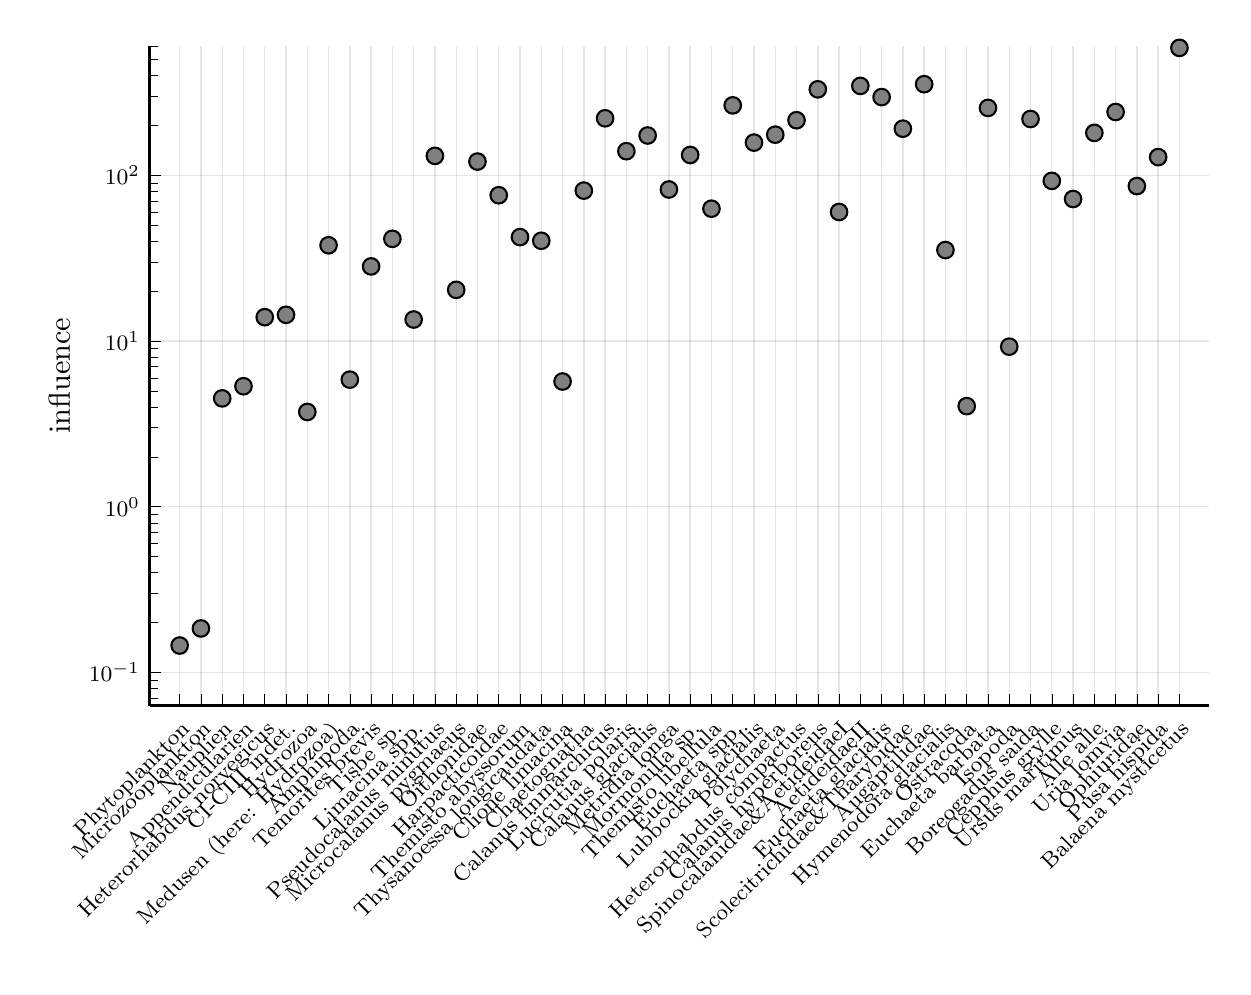
\begin{tikzpicture}[/tikz/background rectangle/.style={fill={rgb,1:red,1.0;green,1.0;blue,1.0}, fill opacity={1.0}, draw opacity={1.0}}, show background rectangle]
\begin{axis}[ymode = log, point meta max={nan}, point meta min={nan}, legend cell align={left}, legend columns={1}, title={}, title style={at={{(0.5,1)}}, anchor={south}, font={{\fontsize{14 pt}{18.2 pt}\selectfont}}, color={rgb,1:red,0.0;green,0.0;blue,0.0}, draw opacity={1.0}, rotate={0.0}, align={center}}, legend style={color={rgb,1:red,0.0;green,0.0;blue,0.0}, draw opacity={1.0}, line width={1}, solid, fill={rgb,1:red,1.0;green,1.0;blue,1.0}, fill opacity={1.0}, text opacity={1.0}, font={{\fontsize{8 pt}{10.4 pt}\selectfont}}, text={rgb,1:red,0.0;green,0.0;blue,0.0}, cells={anchor={center}}, at={(1.02, 1)}, anchor={north west}}, axis background/.style={fill={rgb,1:red,1.0;green,1.0;blue,1.0}, opacity={1.0}}, anchor={north west}, xshift={1.0mm}, yshift={-1.0mm}, width={150.4mm}, height={99.6mm}, scaled x ticks={false}, xlabel={}, x tick style={color={rgb,1:red,0.0;green,0.0;blue,0.0}, opacity={1.0}}, x tick label style={color={rgb,1:red,0.0;green,0.0;blue,0.0}, opacity={1.0}, rotate={45}}, xlabel style={at={(ticklabel cs:0.5)}, anchor=near ticklabel, at={{(ticklabel cs:0.5)}}, anchor={near ticklabel}, font={{\fontsize{11 pt}{14.3 pt}\selectfont}}, color={rgb,1:red,0.0;green,0.0;blue,0.0}, draw opacity={1.0}, rotate={0.0}}, xmajorgrids={true}, xmin={-0.41000000000000014}, xmax={49.41}, xticklabels={{Phytoplankton ,Microzooplankton,Nauplien ,Appendicularien,Heterorhabdus norvegicus,CI-CIII indet.,Hydrozoa,Medusen (here: Hydrozoa),Amphipoda,Temorites brevis,Tisbe sp.,Limacina spp. ,Pseudocalanus minutus,Microcalanus pygmaeus,Oithonidae,Harpacticoidae ,Themisto abyssorum,Thysanoessa longicaudata,Clione limacina,Chaetognatha,Calanus finmarchicus,Lucicutia polaris,Calanus glacialis,Metridia longa,Mormonilla sp.,Themisto libellula,Euchaeta spp.,Lubbockia glacialis,Polychaeta,Heterorhabdus compactus,Calanus hyperboreus,Spinocalanidae\&AetideidaeI,AetideidaeII,Euchaeta glacialis,Scolecitrichidae\&Tharybidae,Augaptilidae,Hymenodora glacialis,Ostracoda,Euchaeta barbata ,Isopoda,Boreogadus saida,Cepphus grylle,Ursus maritimus,Alle alle,Uria lomvia,Ophiuridae,Pusa hispida,Balaena mysticetus}}, xtick={{1,2,3,4,5,6,7,8,9,10,11,12,13,14,15,16,17,18,19,20,21,22,23,24,25,26,27,28,29,30,31,32,33,34,35,36,37,38,39,40,41,42,43,44,45,46,47,48}}, xtick align={inside}, xticklabel style={font={{\fontsize{8 pt}{10.4 pt}\selectfont}}, color={rgb,1:red,0.0;green,0.0;blue,0.0}, draw opacity={1.0}, rotate={0.0}, anchor={north east}}, x grid style={color={rgb,1:red,0.0;green,0.0;blue,0.0}, draw opacity={0.1}, line width={0.5}, solid}, axis x line*={left}, x axis line style={color={rgb,1:red,0.0;green,0.0;blue,0.0}, draw opacity={1.0}, line width={1}, solid}, scaled y ticks={false}, ylabel={influence}, y tick style={color={rgb,1:red,0.0;green,0.0;blue,0.0}, opacity={1.0}}, y tick label style={color={rgb,1:red,0.0;green,0.0;blue,0.0}, opacity={1.0}, rotate={0}}, ylabel style={at={(ticklabel cs:0.5)}, anchor=near ticklabel, at={{(ticklabel cs:0.5)}}, anchor={near ticklabel}, font={{\fontsize{11 pt}{14.3 pt}\selectfont}}, color={rgb,1:red,0.0;green,0.0;blue,0.0}, draw opacity={1.0}, rotate={0.0}}, ymajorgrids={true}, ymin={-17.465794460399593}, ymax={604.7988898814917},
%	 yticklabels={{$0$,$100$,$200$,$300$,$400$,$500$,$600$}}, ytick={{0.0,100.0,200.0,300.0,400.0,500.0,600.0}}, 
	 ytick align={inside}, yticklabel style={font={{\fontsize{8 pt}{10.4 pt}\selectfont}}, color={rgb,1:red,0.0;green,0.0;blue,0.0}, draw opacity={1.0}, rotate={0.0}}, y grid style={color={rgb,1:red,0.0;green,0.0;blue,0.0}, draw opacity={0.1}, line width={0.5}, solid}, axis y line*={left}, y axis line style={color={rgb,1:red,0.0;green,0.0;blue,0.0}, draw opacity={1.0}, line width={1}, solid}, colorbar={false}]
    \addplot[color={rgb,1:red,0.502;green,0.502;blue,0.502}, name path={18}, only marks, draw opacity={1.0}, line width={0}, solid, mark={*}, mark size={3.0 pt}, mark repeat={1}, mark options={color={rgb,1:red,0.0;green,0.0;blue,0.0}, draw opacity={1.0}, fill={rgb,1:red,0.502;green,0.502;blue,0.502}, fill opacity={1.0}, line width={0.75}, rotate={0}, solid}]
        table[row sep={\\}]
        {
            \\
            1.0  0.14547019078601167  \\
            2.0  0.1844751735766008  \\
            3.0  4.5088799790655445  \\
            4.0  5.338402263049102  \\
            5.0  13.926163362150048  \\
            6.0  14.396475369484767  \\
            7.0  3.733648269400605  \\
            8.0  37.822981202625684  \\
            9.0  5.848987089533179  \\
            10.0  28.200941627384264  \\
            11.0  41.365890673913164  \\
            12.0  13.483693798485472  \\
            13.0  130.99197033888495  \\
            14.0  20.364280776414148  \\
            15.0  120.96880971564862  \\
            16.0  75.82943338043737  \\
            17.0  42.386816177395396  \\
            18.0  40.25968556388621  \\
            19.0  5.69820974873087  \\
            20.0  80.859937576482  \\
            21.0  220.74537548174072  \\
            22.0  139.75054407283827  \\
            23.0  173.86126368470676  \\
            24.0  82.10677752628094  \\
            25.0  132.6321444160116  \\
            26.0  62.88080189892516  \\
            27.0  264.22756898404907  \\
            28.0  157.4937111037753  \\
            29.0  175.8972151403554  \\
            30.0  214.86158764843609  \\
            31.0  330.15600477840815  \\
            32.0  60.06820659562924  \\
            33.0  346.2498365815547  \\
            34.0  296.30951775886916  \\
            35.0  191.09716683979966  \\
            36.0  354.50760102202787  \\
            37.0  35.39969989806317  \\
            38.0  4.049105009579034  \\
            39.0  255.04080187359742  \\
            40.0  9.245804057666605  \\
            41.0  218.6575470747945  \\
            42.0  92.54120112299898  \\
            43.0  71.94016343254172  \\
            44.0  180.27006808326414  \\
            45.0  240.9786157212713  \\
            46.0  86.13881607563897  \\
            47.0  128.74757875215124  \\
            48.0  587.1876252303061  \\
        }
        ;
\end{axis}
\end{tikzpicture}

	}
	\caption{
		Influence of each species.
	}
\end{figure}

\end{document}